\section{Data}
\label{sec:data}

All series were retrieved from the Federal Reserve Bank of St.\ Louis (FRED); the originating agencies are listed in Table~\ref{tab:variables}. The panel is quarterly and runs from 1959 through 2026 where series permit. Series reported at higher frequencies are converted to quarterly by averaging within the quarter for interest rates and price indices and by taking the end-of-quarter value for stocks. Series from the Financial Accounts of the United States (Z.1) and the National Income and Product Accounts (NIPA) are already quarterly.

We construct three groups of derived variables. Broad money net of base money is M2 less the monetary base, both in billions of dollars. Inflation is measured as the annualized quarterly log difference of each price index and, where noted, as its year-over-year change. Sectoral interest rates are constructed as interest payments divided by the corresponding stock of debt, which yields a weighted-average rate for the federal, state and local, business, and consumer sectors; for state and local governments we net out the imputed interest on public-pension liabilities that NIPA includes in interest payments, and for mortgages we use the market thirty-year fixed rate because long mortgage durations make the current rate more informative than a weighted average. We use market interest rates for the same sectors as a robustness comparison.

Because this is a time-series study, we present the series as plots rather than as conventional summary statistics. Figures~\ref{fig:money} through~\ref{fig:fed} show the money supply, inflation, sectoral debt, interest rates, and the Federal Reserve balance sheet, and Figure~\ref{fig:impliedvsmarket} compares the implied and market rates by sector.

\section{Money Supply and Inflation}
\label{sec:money_inflation}

We first evaluate the link between money and inflation with a trivariate vector autoregression (VAR) in real output growth, the growth of M2 less the monetary base, and inflation. Augmented Dickey--Fuller and KPSS tests (Table~\ref{tab:unitroots}) indicate that the log levels are integrated of order one while growth rates and inflation are treated as stationary. We select the lag length by the Akaike information criterion, capped at eight lags, confirm that all inverse roots lie inside the unit circle, and report Granger-causality tests, orthogonalized impulse responses under a recursive ordering that places output first and prices last, and the associated forecast-error variance decomposition.

Table~\ref{tab:task1} collects the results for the four inflation measures. Over the full sample the evidence that money growth Granger-causes inflation is marginal, and before the pandemic the stronger direction runs from inflation to money. In the short post-2020 window the share of inflation forecast-error variance attributable to money shocks is larger, but this sample is only twenty-five quarters and we do not rest inference on it. Figure~\ref{fig:task1irf} shows the impulse response of inflation to a money-growth shock, and Figure~\ref{fig:rollgranger} shows how the money-inflation relationship moves over time in a rolling window.

\section{The Interest-Rate System}
\label{sec:rates}

We next examine how the five sectoral interest rates respond to the money supply and to one another. The appropriate specification depends on cointegration, which we assess with Johansen trace tests in both levels and differences (Table~\ref{tab:johansen}). The implied rates are not cointegrated in levels, so we estimate that system as a VAR in first differences (Table~\ref{tab:ratehier_implied}). The market rates are cointegrated, so we model them with a vector error-correction model (VECM) instead (Table~\ref{tab:ratehier_market}); differencing a cointegrated system would discard the long-run relationships. Because interest rates are highly persistent, we confirm the causal ordering with lag-augmented (Toda--Yamamoto) tests as well.

In the correctly specified market-rate VECM the federal rate Granger-causes the other rates while the reverse is insignificant, giving a one-way hierarchy consistent with monetary policy moving rates across the term structure. In the differenced implied-rate system the federal rate still leads the others, though feedback is present. Figure~\ref{fig:heatmap} summarizes the pairwise Granger-causality pattern. The contrast between the cointegrated market rates and the non-cointegrated implied rates is itself a result: policy moves market rates together, but realized borrowing costs across sectors do not share a single long-run trend, which points to differences in borrower behavior across sectors.

\section{Federal Reserve Transactions}
\label{sec:fed}

To identify the role of central-bank policy, we estimate a six-variable system in Federal Reserve securities growth, base-money growth, the growth of M2 less base, the change in the funds rate, the change in the ten-year yield, and CPI inflation, from 2003 onward (the balance-sheet series begin in late 2002). Table~\ref{tab:task4granger} reports the Granger tests. Federal Reserve purchases drive the monetary base throughout, and before the pandemic they also drive broad money and the funds rate. Once the pandemic quarters enter, the channel from purchases to broad money weakens, consistent with the pandemic-era expansion of M2 arising through fiscal rather than open-market operations. Johansen tests indicate cointegration, so we also estimate a VECM; Table~\ref{tab:task4vecm} reports both deterministic specifications together with residual diagnostics, and Figure~\ref{fig:task4irf} shows the responses to a securities-purchase shock.

\section{The Demand for Loanable Funds}
\label{sec:loanable}

Finally we ask what is driving the demand for loanable funds. Table~\ref{tab:task5period} compares period averages before, during, and after the pandemic, and Figure~\ref{fig:shares} plots the components of nominal output; consumption's share is essentially flat, so the higher demand for funds is broad-based borrowing rather than a shift toward consumption. We then estimate time-varying-coefficient regressions of each sector's borrowing growth on its own interest rate and lagged money growth, using both a Kalman-smoothed random-walk coefficient model and a rolling ordinary-least-squares window, and under both M2 less base and base money. Table~\ref{tab:task5b} reports the coefficient on money growth by sector, and Figure~\ref{fig:task5b} plots it over time. Consumer borrowing carries a positive coefficient on money growth while business borrowing does not and turns negative after 2020, consistent with a credit-demand mechanism that is weaker where borrowing funds value creation.

\section{Robustness}
\label{sec:robustness}

We assess several threats to the results. Table~\ref{tab:ordering} shows that the variance decompositions are stable across alternative recursive orderings. Table~\ref{tab:inflform} shows that the money-inflation results are insensitive to treating inflation as stationary or as a first difference. Table~\ref{tab:break} reports a Quandt--Andrews sup-Wald test with a bootstrap $p$-value; the dominant structural break in the money-inflation relation is the early-1980s regime change rather than 2020, so we treat the post-2020 evidence as descriptive. Table~\ref{tab:constancy} reports the estimated innovation variance of each time-varying coefficient, which shows that several coefficients are effectively constant while the business money coefficient genuinely varies. Table~\ref{tab:fragility} records which of the headline money-inflation results are statistically fragile.

\clearpage
\section*{Figures}

\begin{figure}[htbp]\centering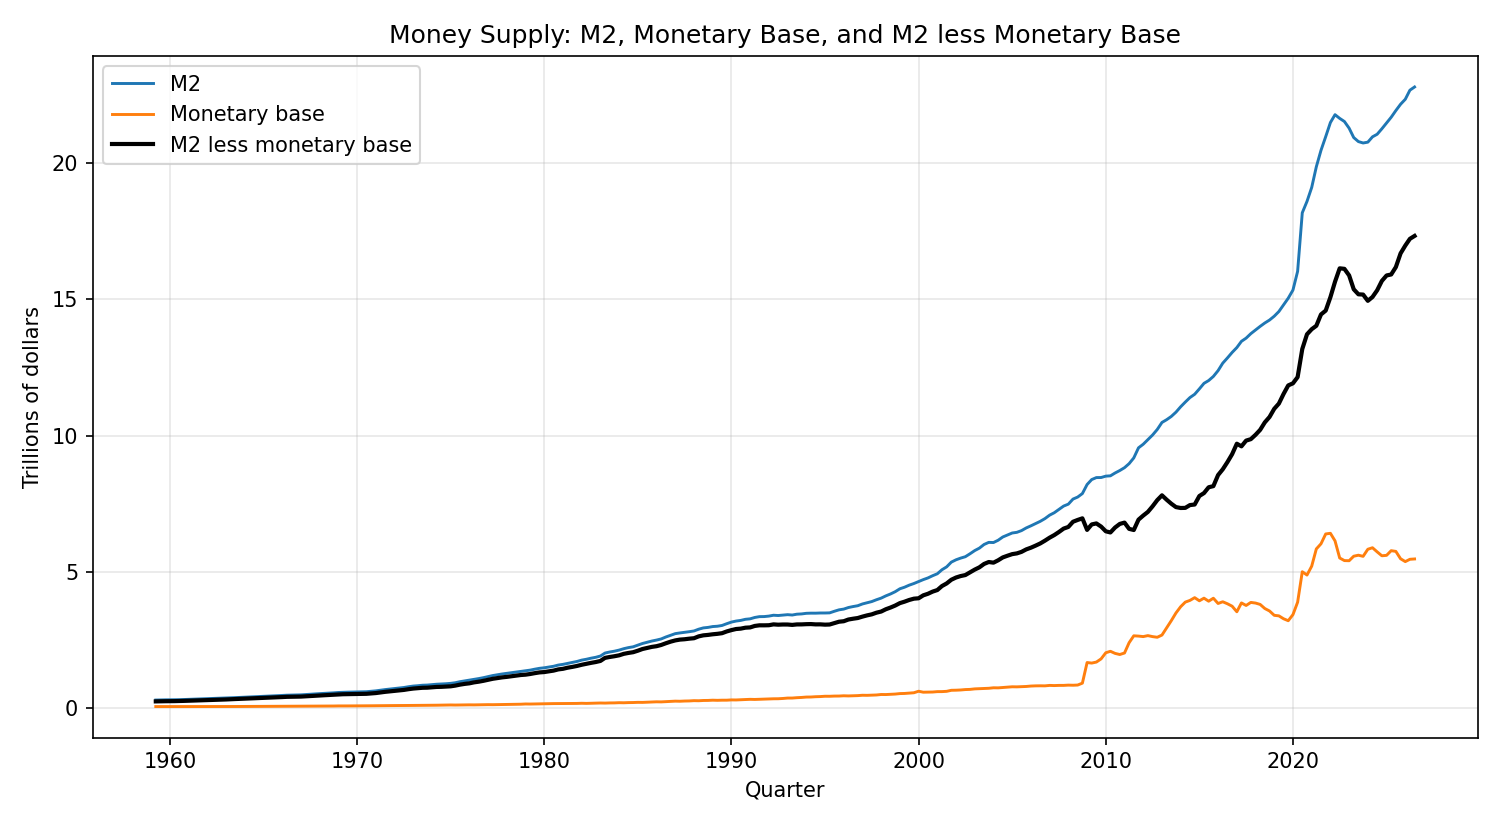
\includegraphics[width=\textwidth]{figures/fig1_money_supply.png}
\caption{M2, the monetary base, and M2 less the monetary base.}\label{fig:money}\end{figure}

\begin{figure}[htbp]\centering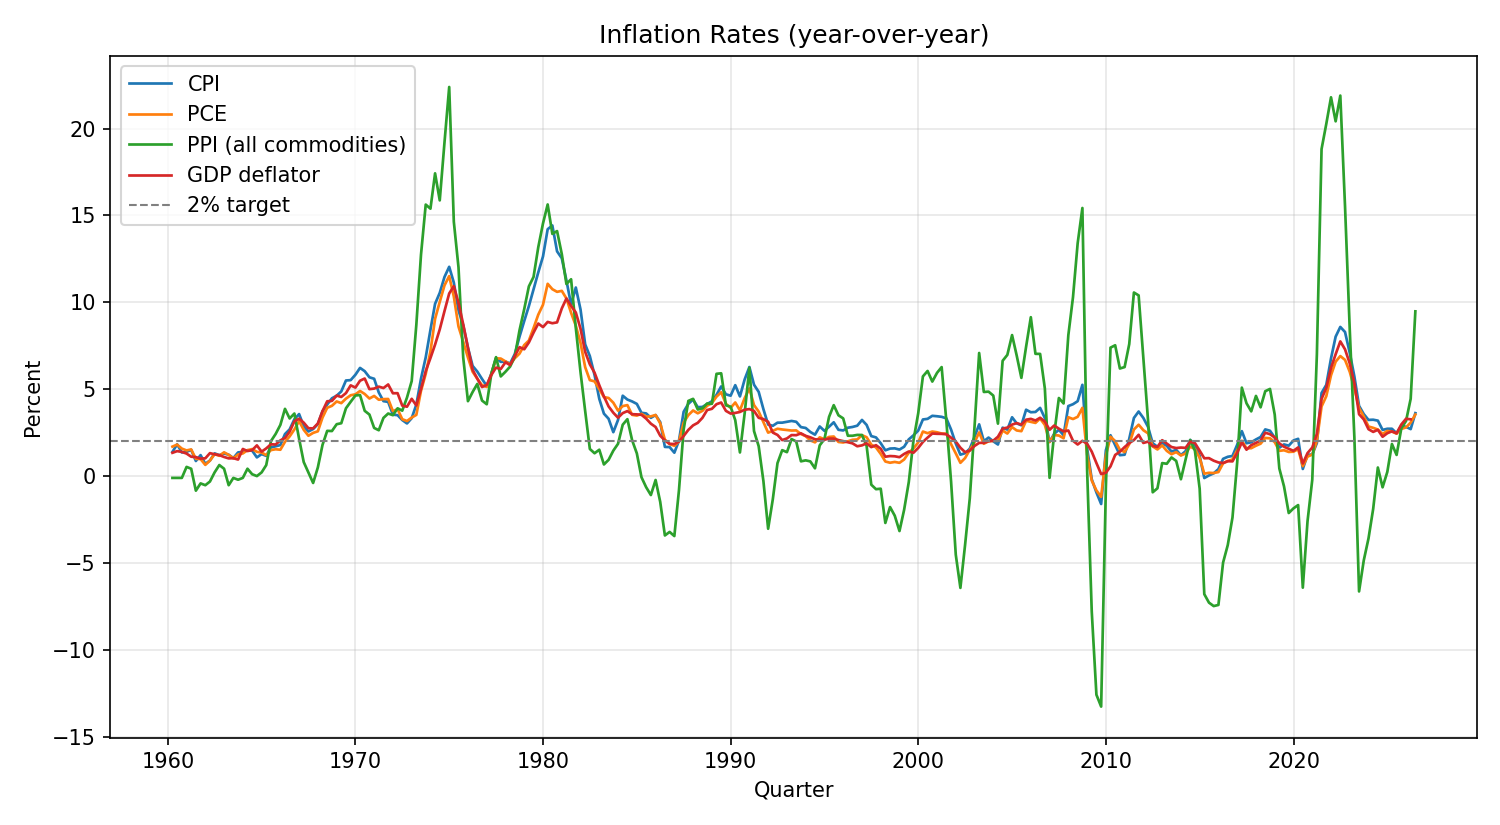
\includegraphics[width=\textwidth]{figures/fig2_inflation.png}
\caption{Inflation rates, year over year.}\label{fig:inflation}\end{figure}

\begin{figure}[htbp]\centering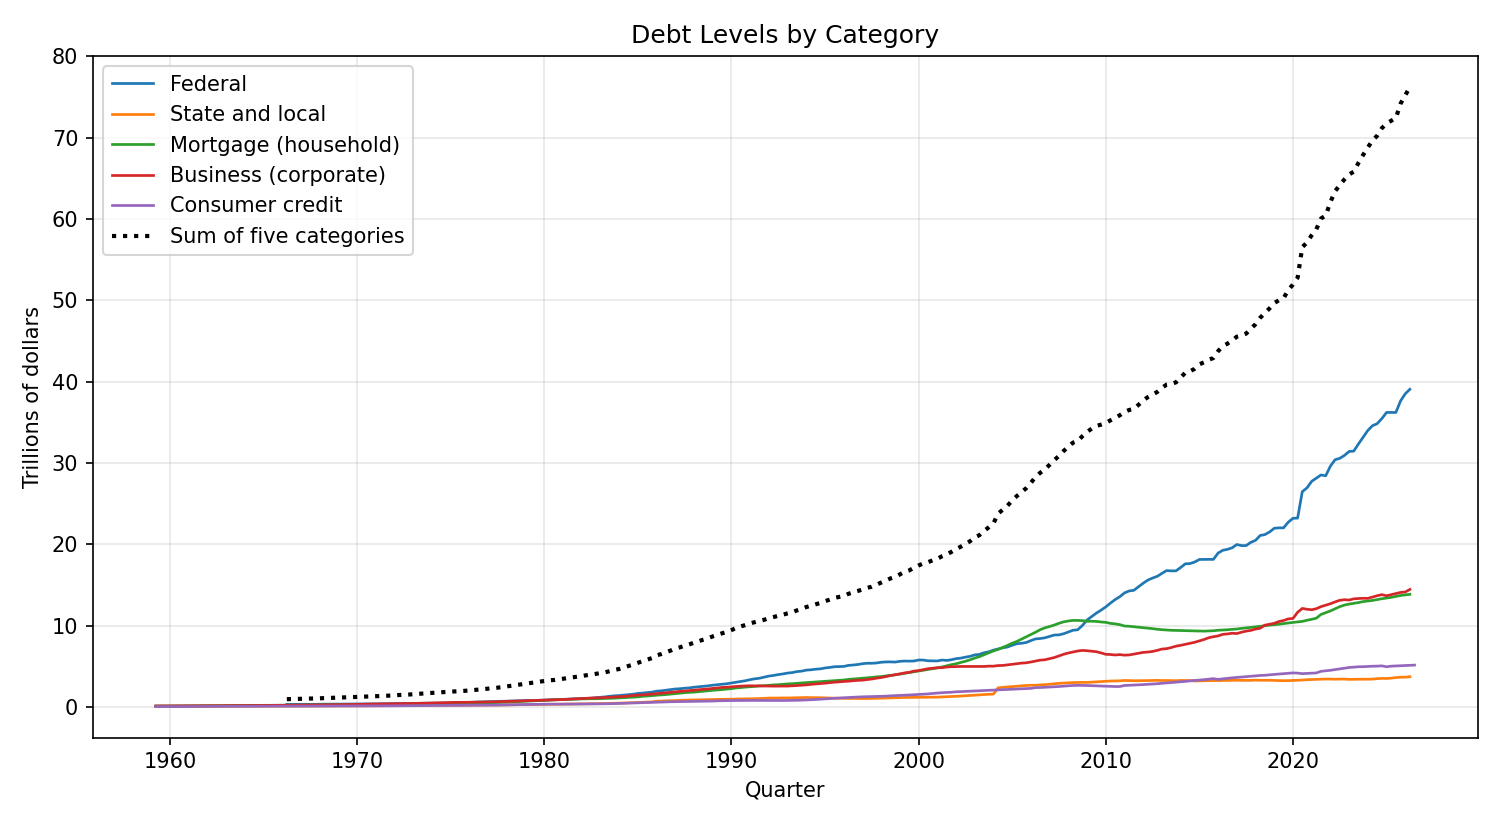
\includegraphics[width=\textwidth]{figures/fig3_debt.png}
\caption{Debt levels by sector.}\label{fig:debt}\end{figure}

\begin{figure}[htbp]\centering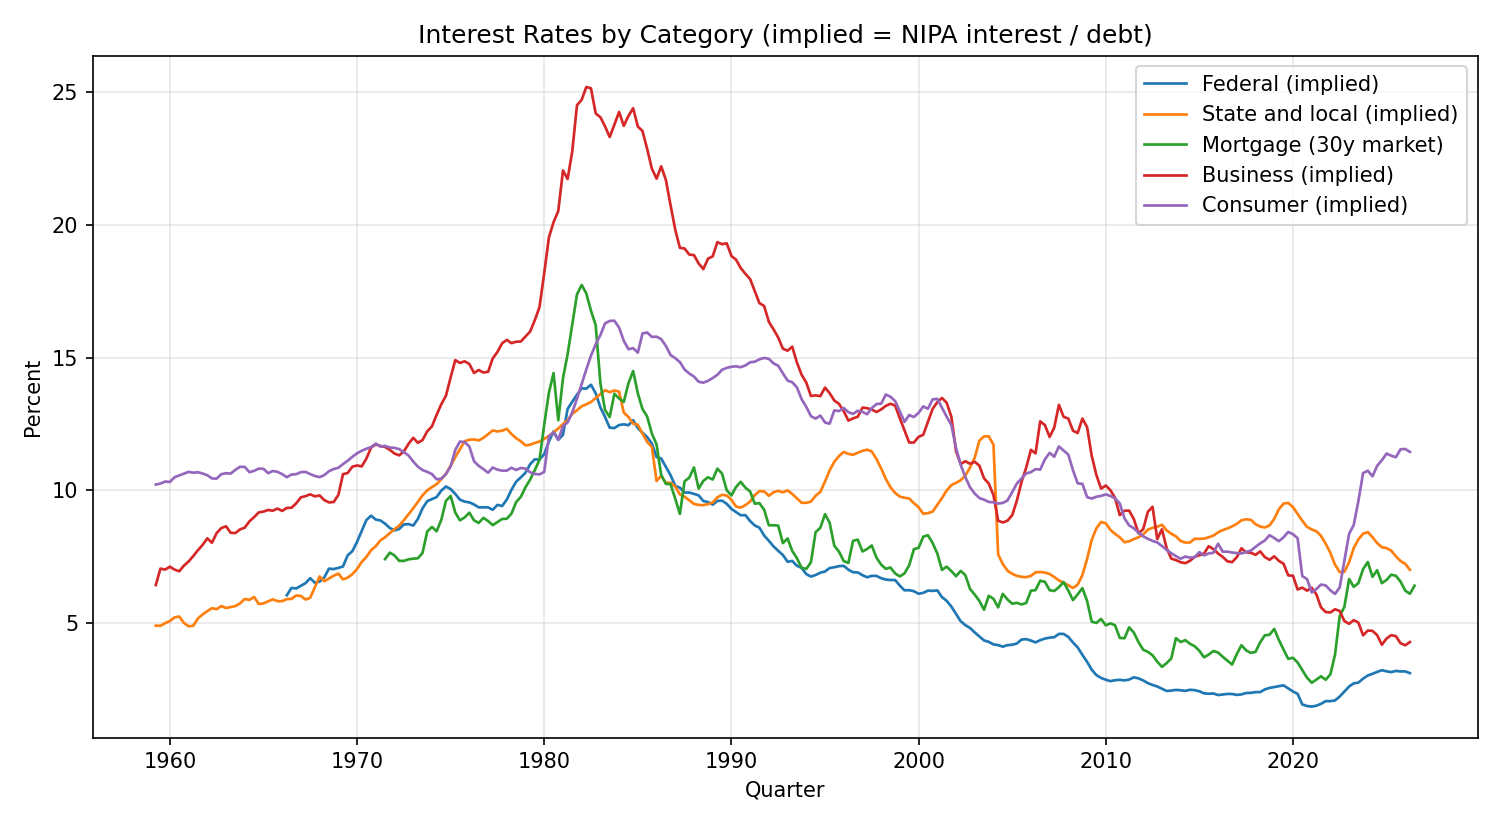
\includegraphics[width=\textwidth]{figures/fig4_interest_rates.png}
\caption{Interest rates by sector.}\label{fig:rates}\end{figure}

\begin{figure}[htbp]\centering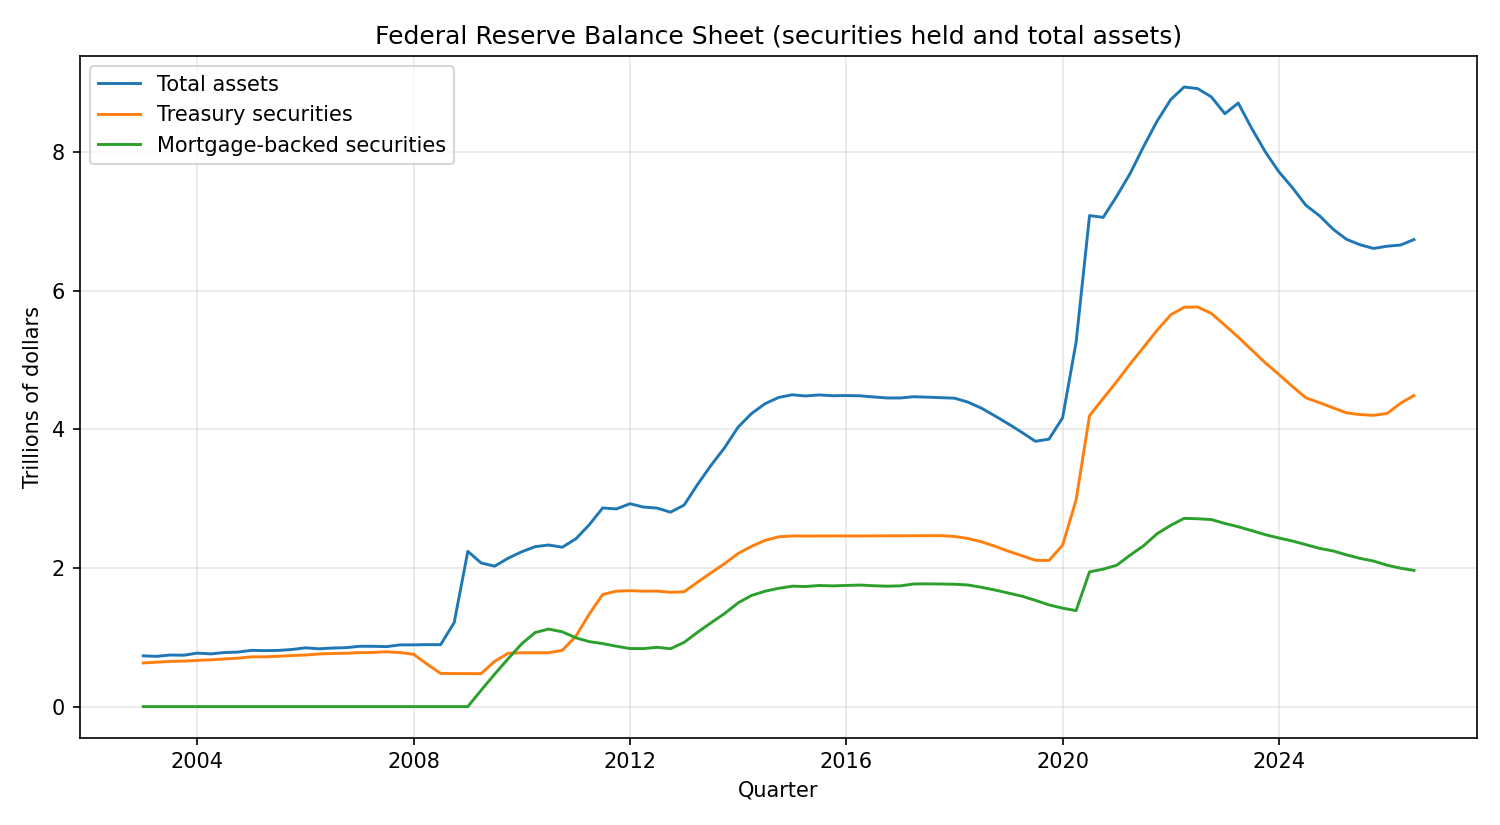
\includegraphics[width=\textwidth]{figures/fig5_fed_balance_sheet.png}
\caption{Federal Reserve balance sheet: total assets, Treasury securities, and mortgage-backed securities.}\label{fig:fed}\end{figure}

\begin{figure}[htbp]\centering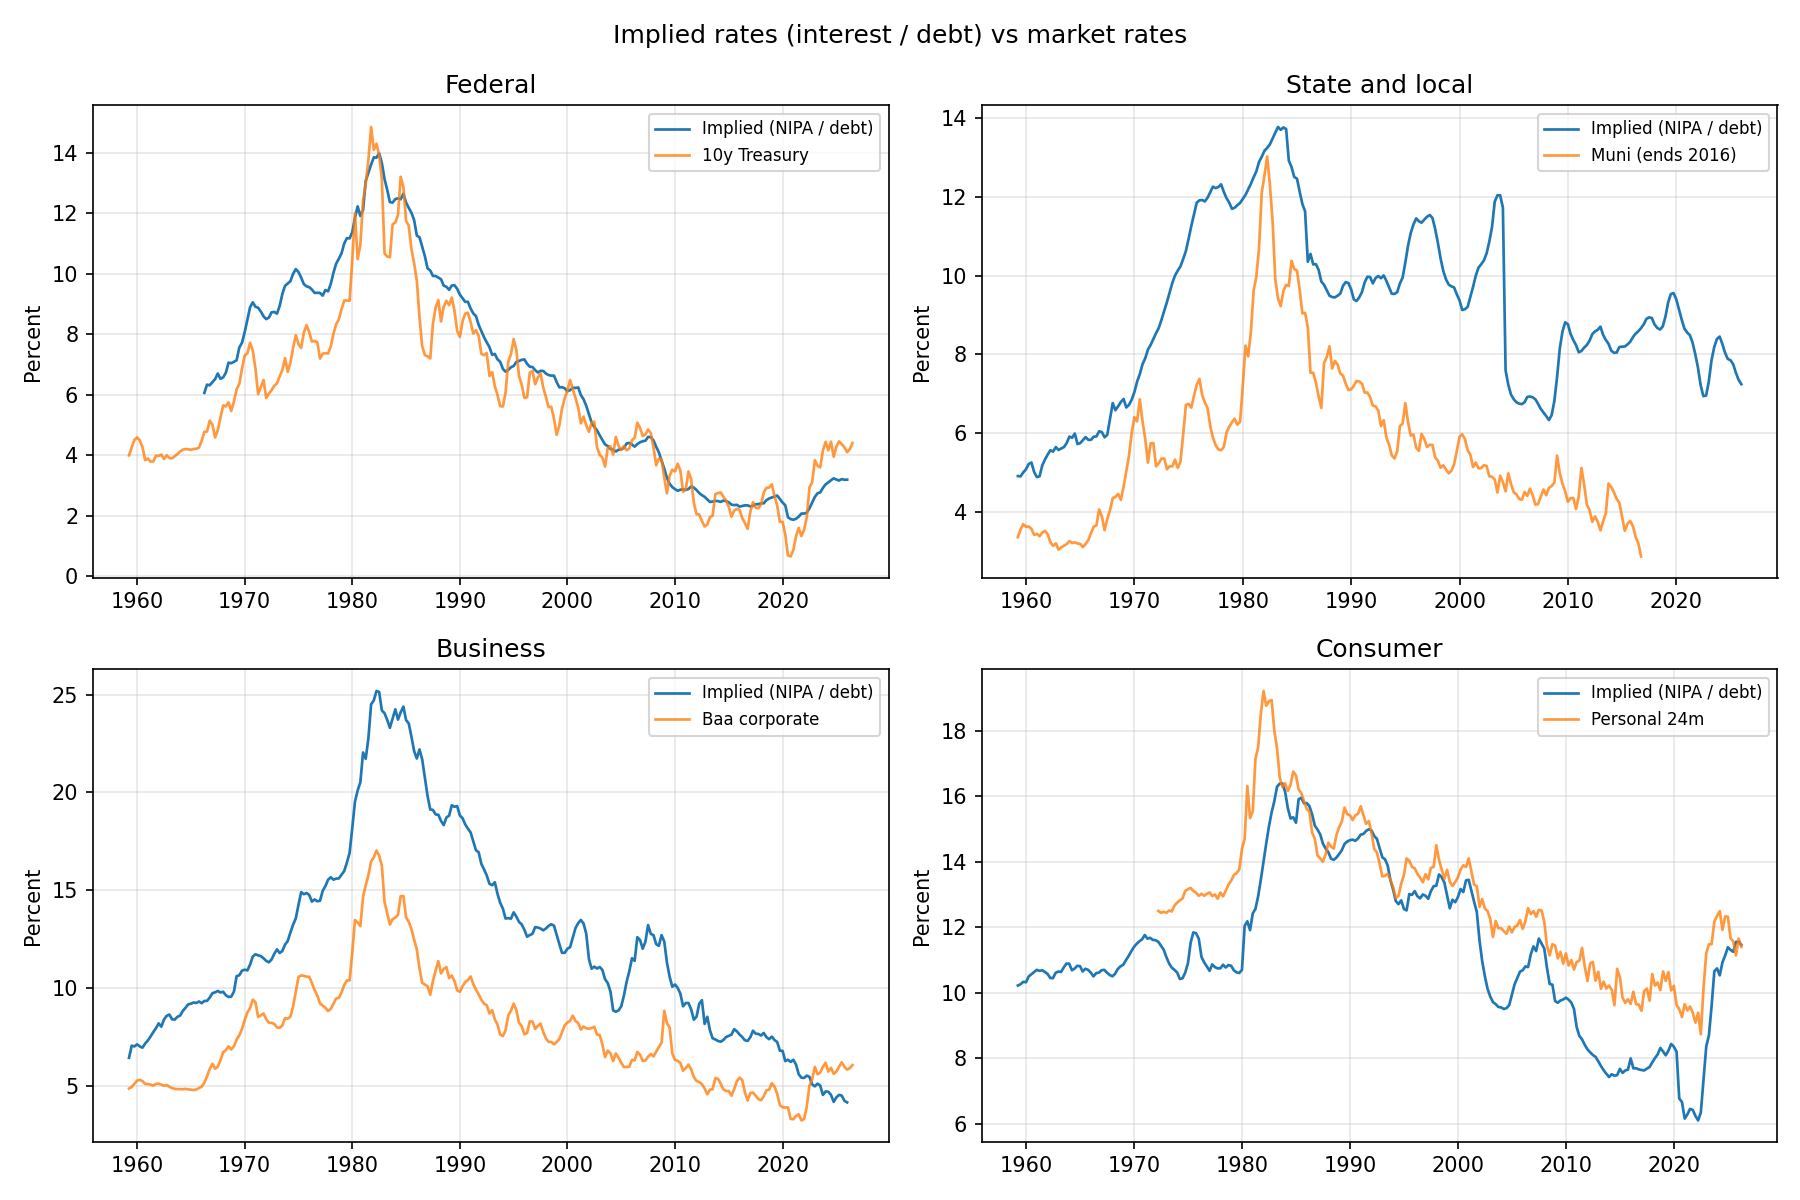
\includegraphics[width=\textwidth]{figures/fig6_implied_vs_market.png}
\caption{Implied sectoral rates (interest over debt) versus market rates.}\label{fig:impliedvsmarket}\end{figure}

\begin{figure}[htbp]\centering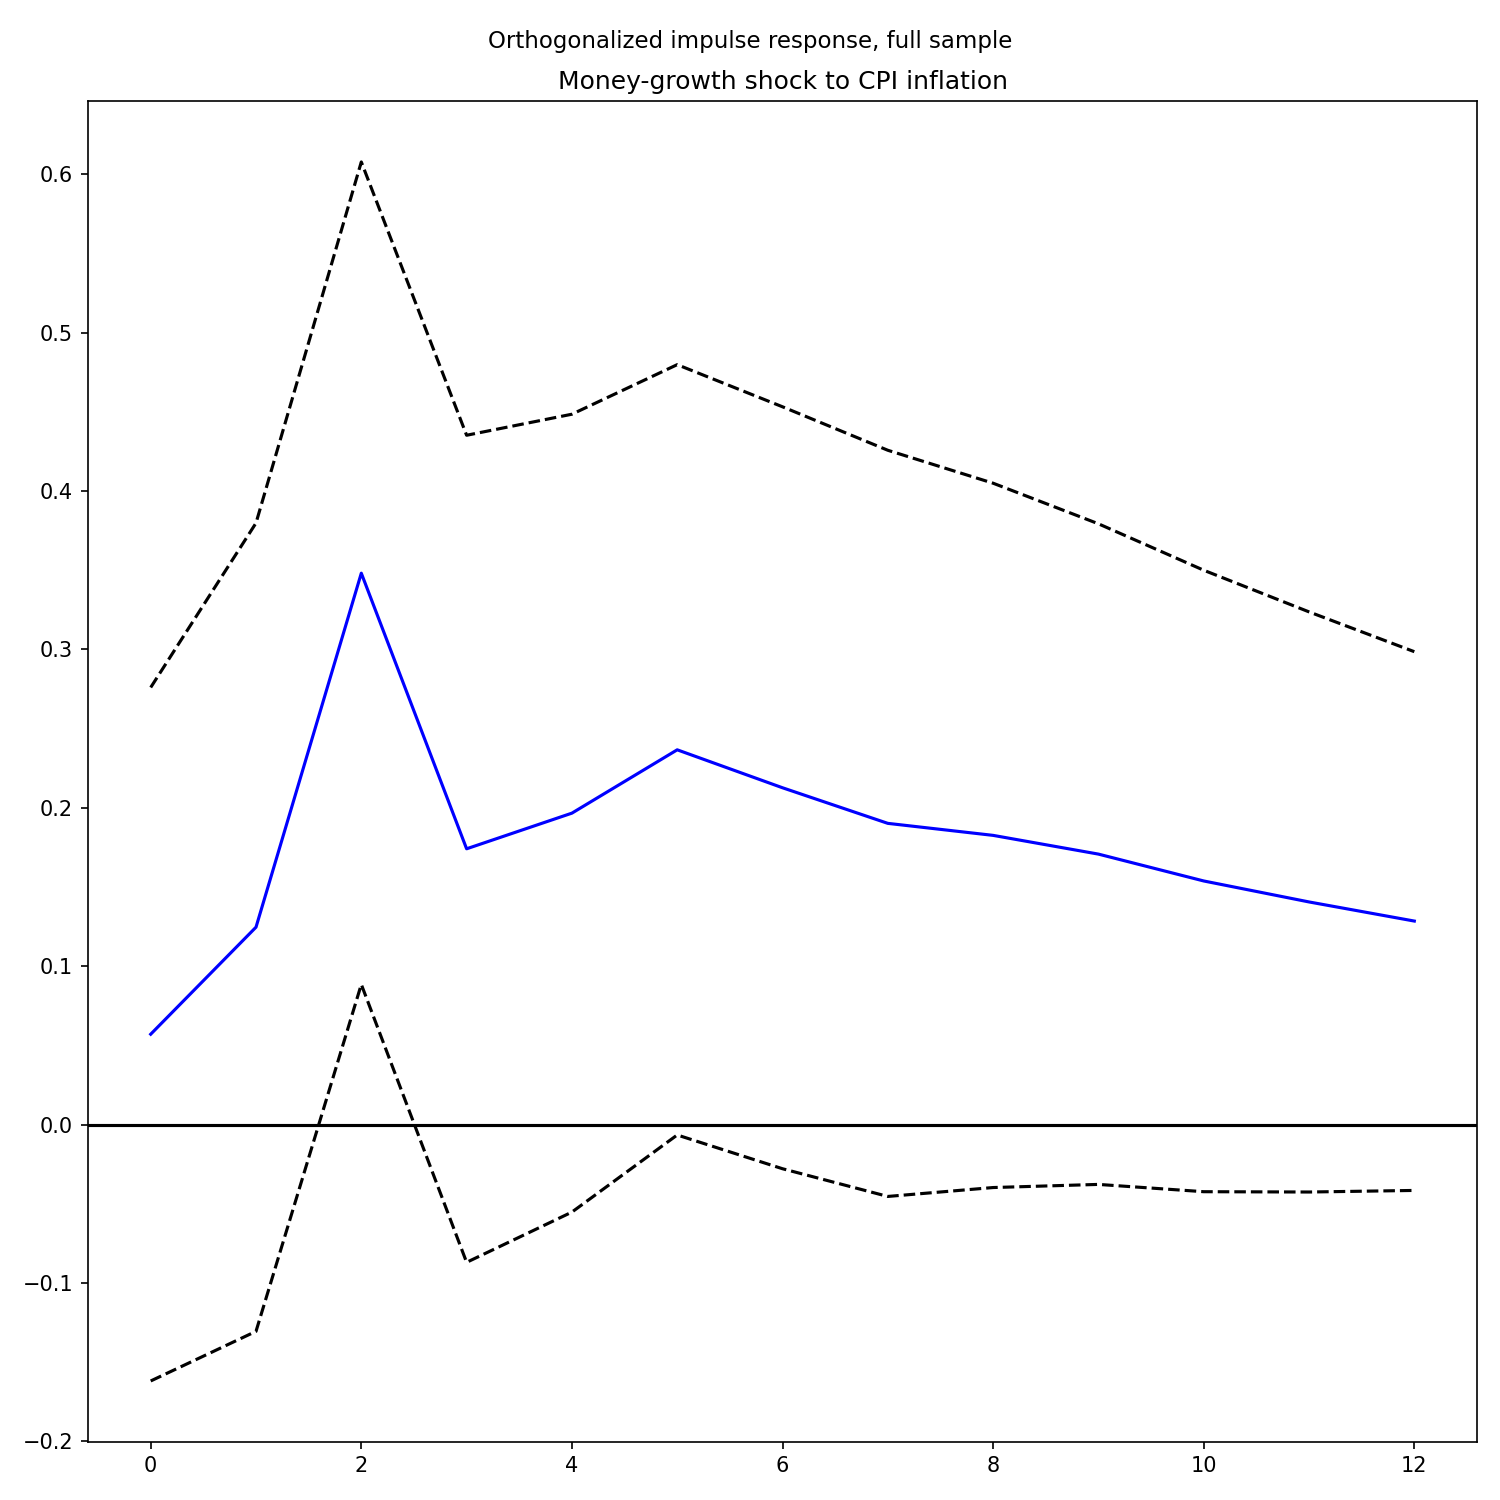
\includegraphics[width=0.9\textwidth]{figures/task1_irf_cpi.png}
\caption{Response of CPI inflation to a one-standard-deviation shock to the growth of M2 less base, with a ninety-five percent band.}\label{fig:task1irf}\end{figure}

\begin{figure}[htbp]\centering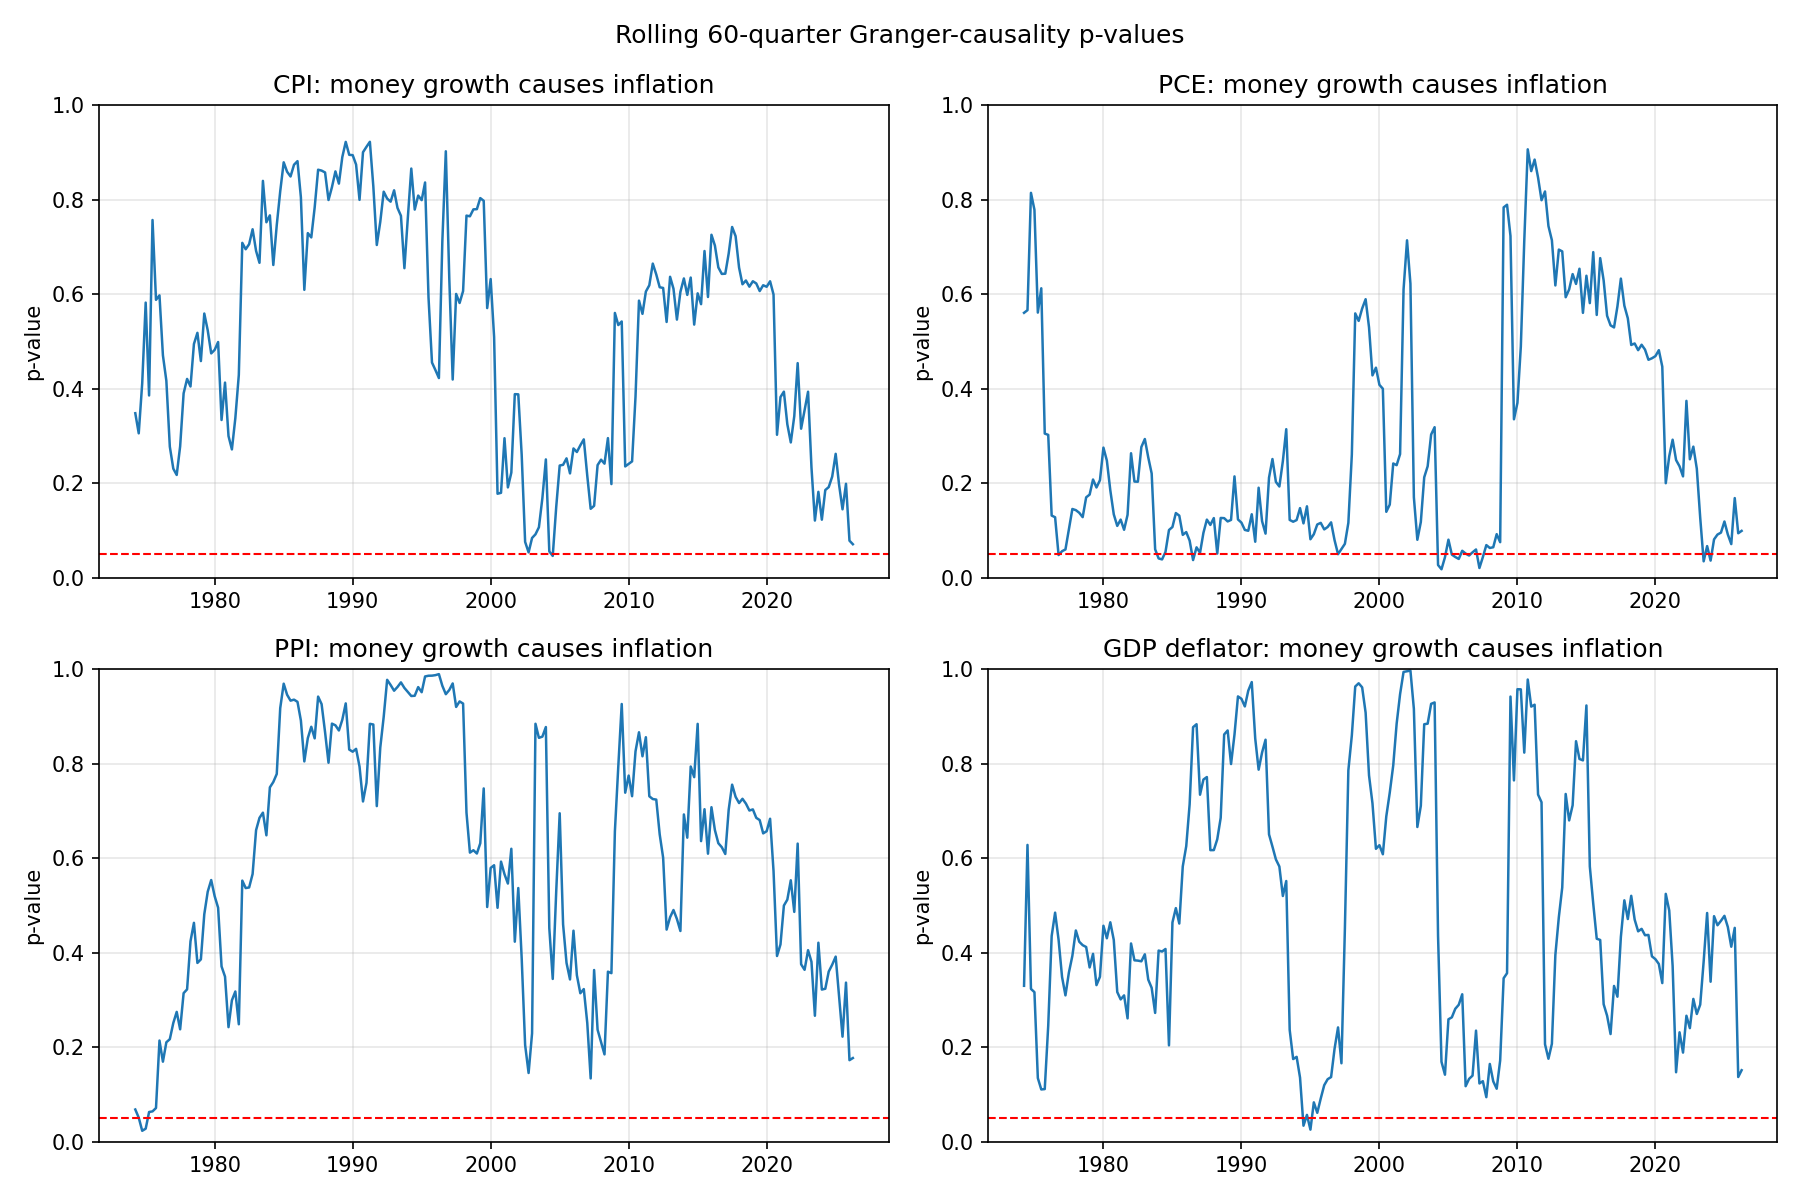
\includegraphics[width=\textwidth]{figures/task1_rolling_granger.png}
\caption{Rolling Granger-causality $p$-values for money growth causing inflation.}\label{fig:rollgranger}\end{figure}

\begin{figure}[htbp]\centering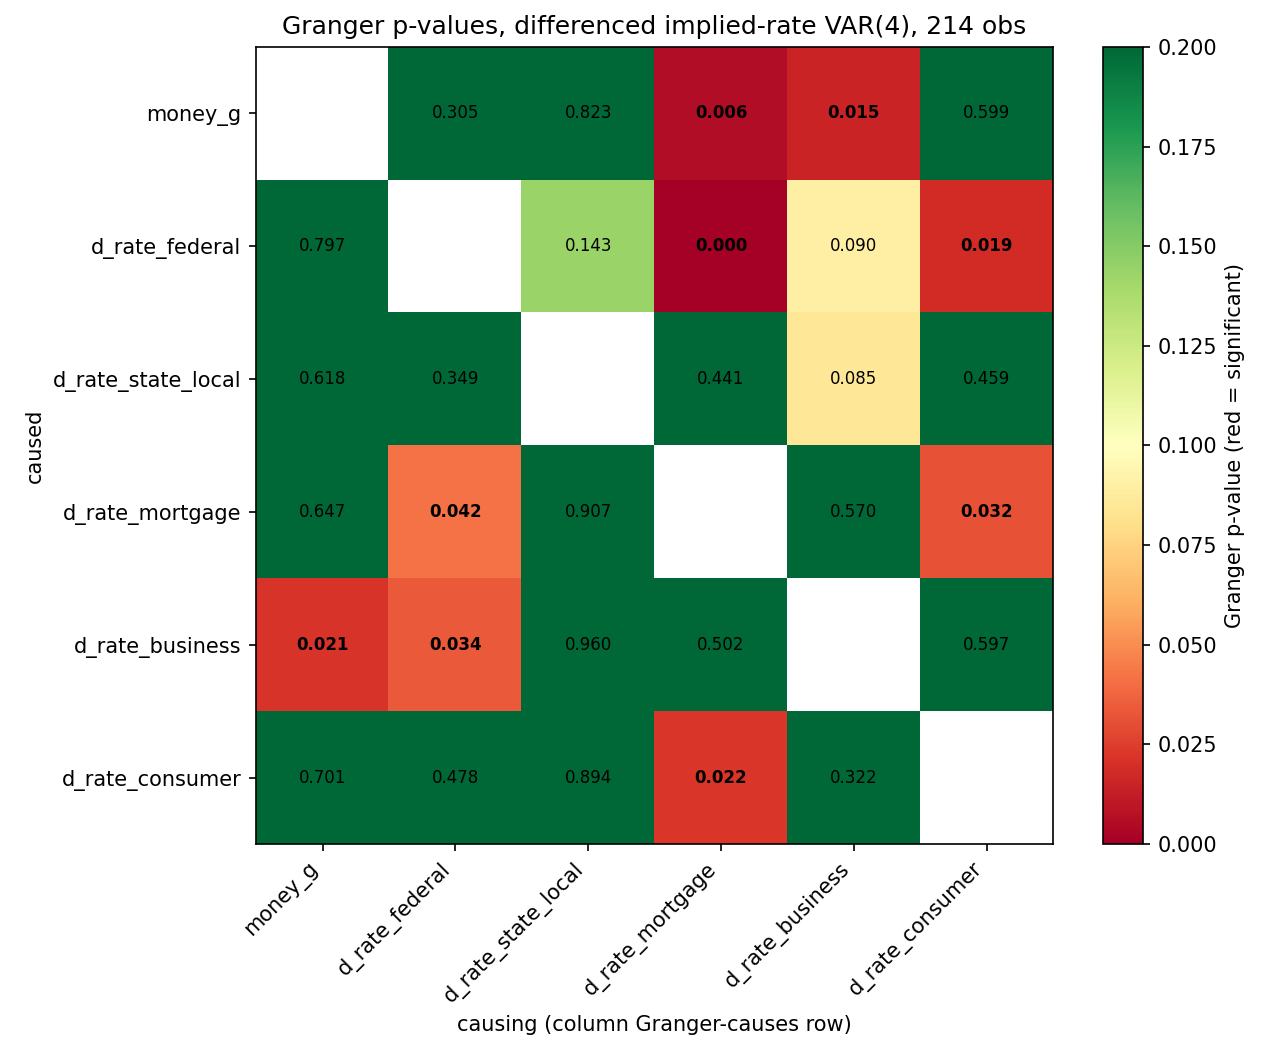
\includegraphics[width=0.85\textwidth]{figures/task23_granger_heatmap.png}
\caption{Granger-causality $p$-values in the differenced implied-rate system.}\label{fig:heatmap}\end{figure}

\begin{figure}[htbp]\centering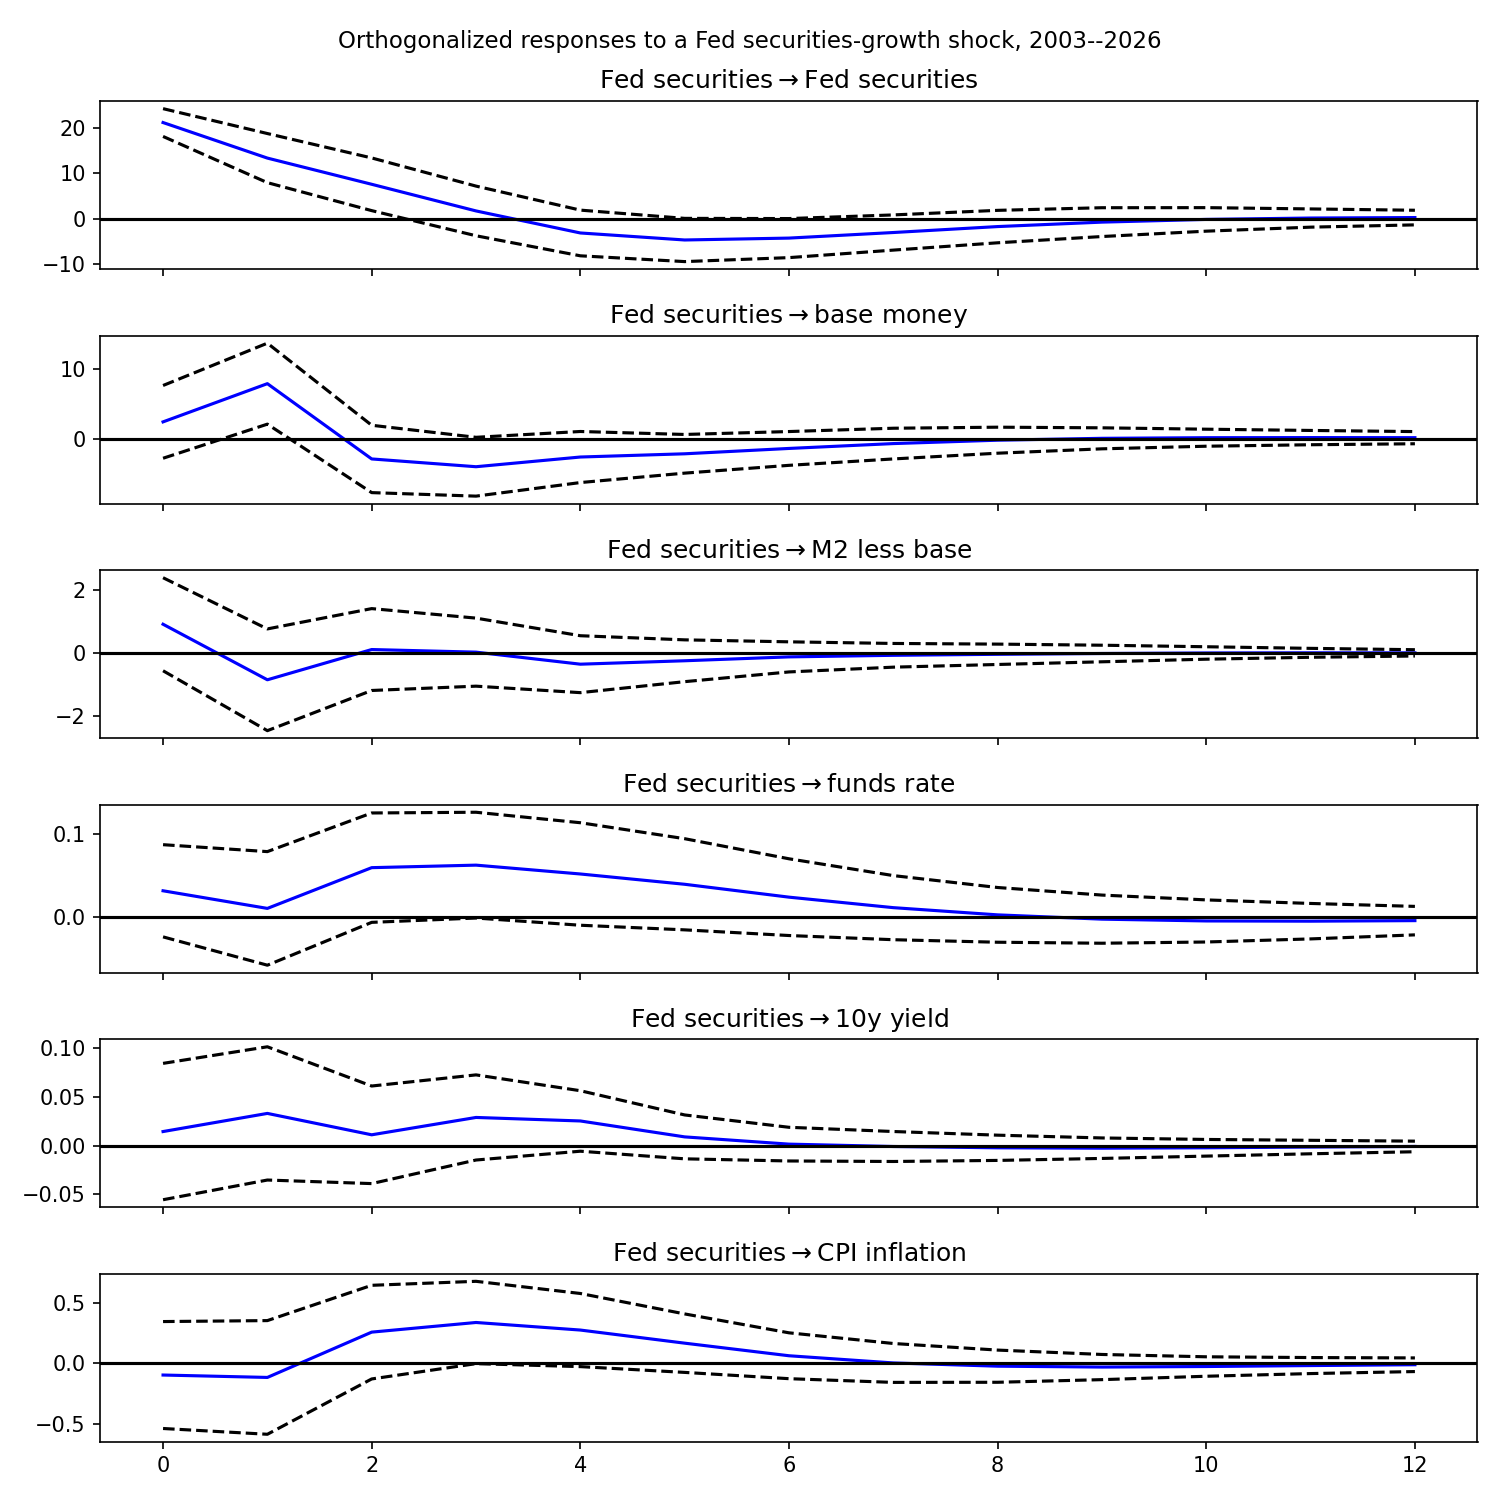
\includegraphics[width=\textwidth]{figures/task4_irf_fed_shock.png}
\caption{Orthogonalized responses to a Federal Reserve securities-growth shock.}\label{fig:task4irf}\end{figure}

\begin{figure}[htbp]\centering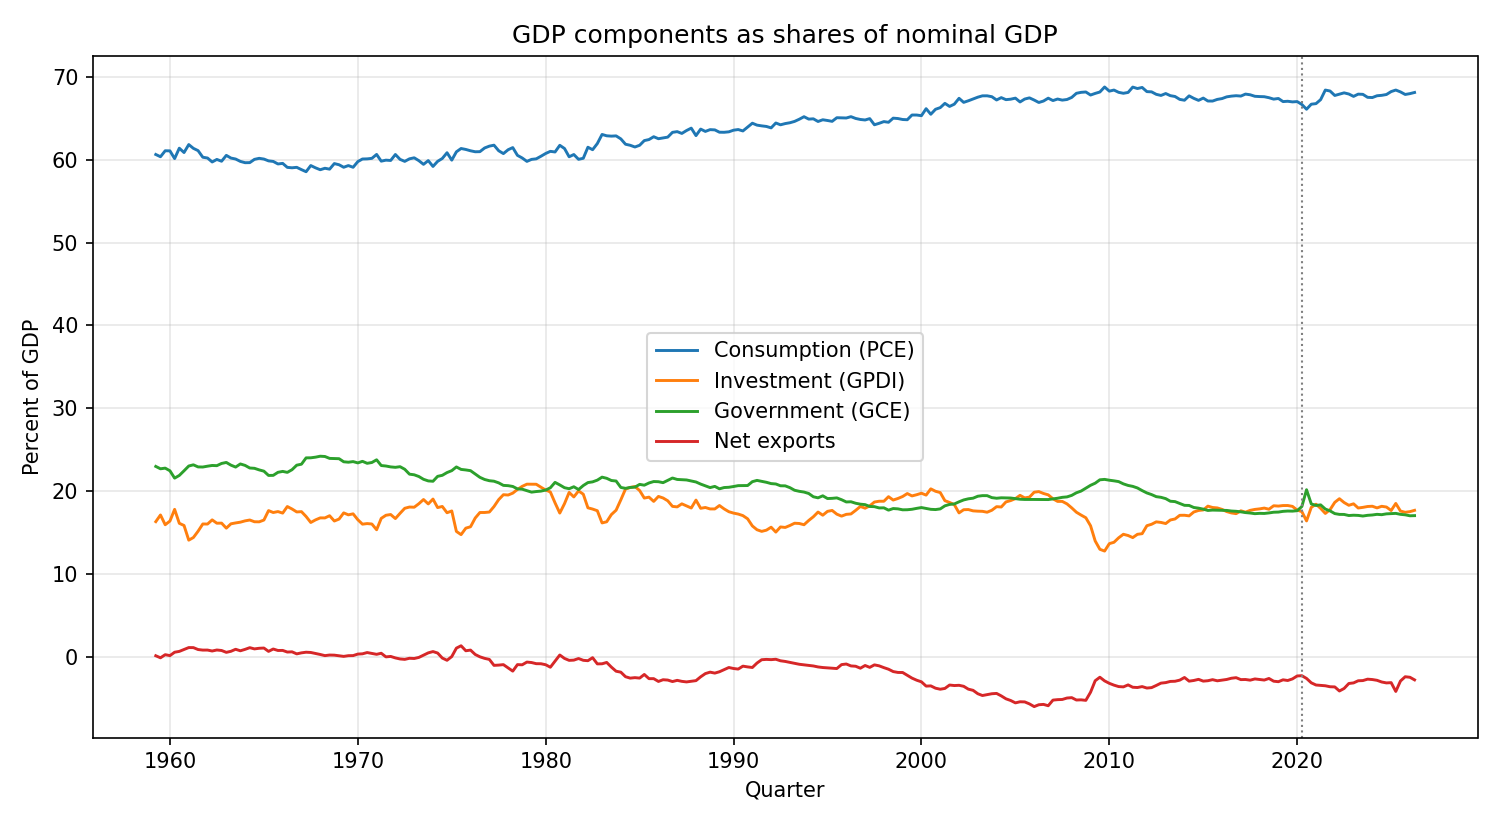
\includegraphics[width=\textwidth]{figures/task5_gdp_shares.png}
\caption{Components of nominal output as shares of GDP.}\label{fig:shares}\end{figure}

\begin{figure}[htbp]\centering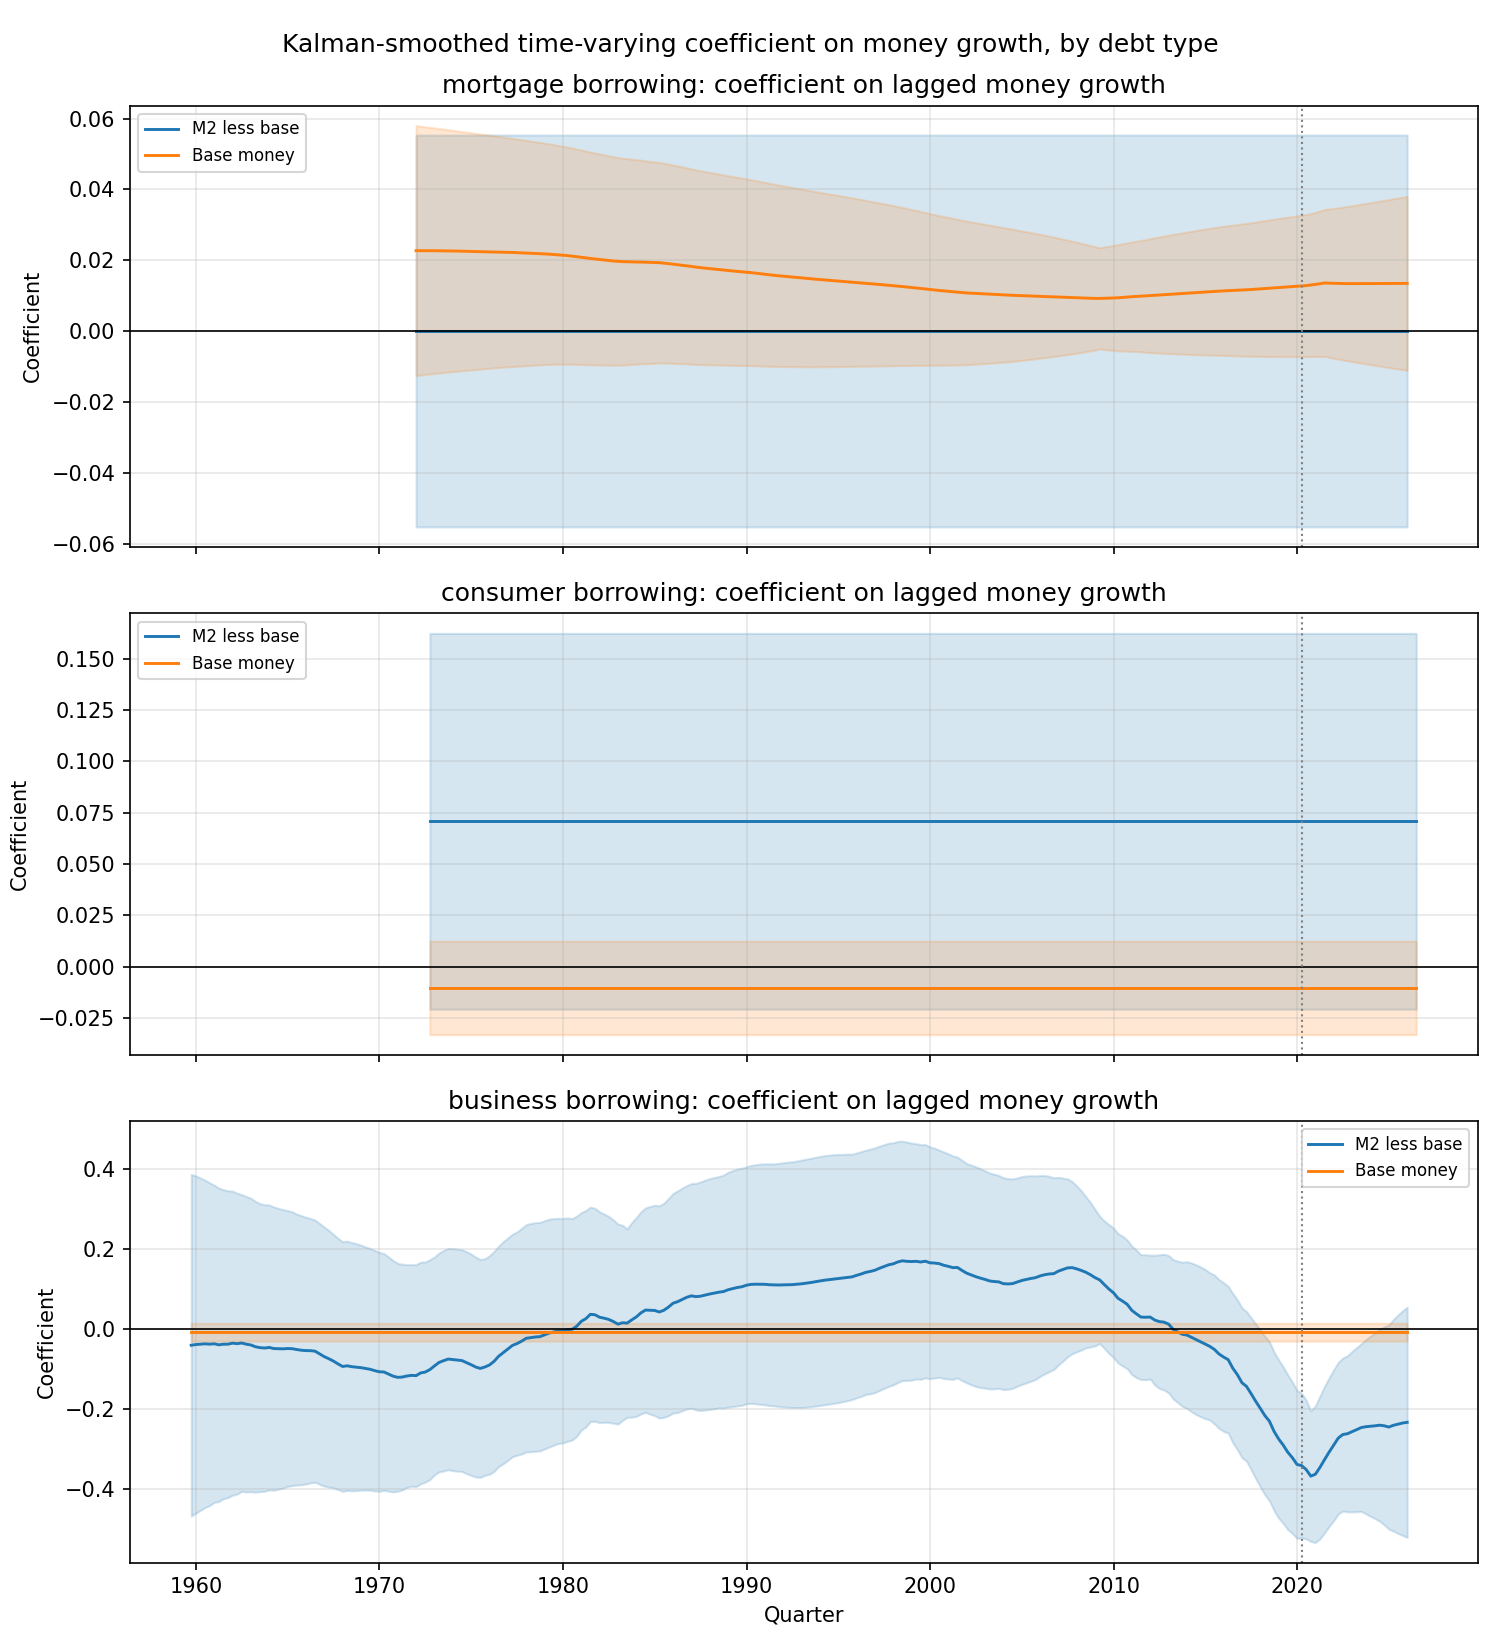
\includegraphics[width=\textwidth]{figures/task5b_tvp_money_coef.png}
\caption{Time-varying coefficient on money growth in each sector's borrowing equation, market rates.}\label{fig:task5b}\end{figure}

\clearpage
\section*{Tables}
\begin{longtable}{@{}llp{5.4cm}llc@{}}
\caption{Variables, units, and sources. All series were retrieved from FRED (Federal Reserve Bank of St.\ Louis); the column ``Source'' gives the originating agency. Coverage is the first and last year available.}\label{tab:variables}\\
\toprule
Variable & Series ID & Description & Units & Source & Coverage \\
\midrule
\endfirsthead
\multicolumn{6}{@{}l}{\emph{Table \ref{tab:variables} continued}}\\
\toprule
Variable & Series ID & Description & Units & Source & Coverage \\
\midrule
\endhead
\midrule \multicolumn{6}{r@{}}{\emph{continued}}\\
\endfoot
\bottomrule
\endlastfoot
\multicolumn{6}{@{}l}{\textbf{Money and reserves}}\\
m2 & M2SL & M2 & Billions of Dollars & Federal Reserve (H.6) & 1959--2026 \\
monetary\_base & BOGMBASE & Monetary Base: Total & Billions of Dollars & Federal Reserve (H.3) & 1959--2026 \\
\addlinespace
\multicolumn{6}{@{}l}{\textbf{Price indices}}\\
cpi & CPIAUCSL & Consumer Price Index for All Urban Consumers: All Items in U.S. City Average & Index 1982-1984=100 & BLS & 1947--2026 \\
pce\_price & PCEPI & Personal Consumption Expenditures: Chain-type Price Index & Index 2017=100 & BEA (NIPA) & 1959--2026 \\
ppi\_allcommodities & PPIACO & Producer Price Index by Commodity: All Commodities & Index 1982=100 & BLS & 1913--2026 \\
gdp\_deflator & GDPDEF & Gross Domestic Product: Implicit Price Deflator & Index 2017=100 & BEA (NIPA) & 1947--2026 \\
\addlinespace
\multicolumn{6}{@{}l}{\textbf{Real output}}\\
real\_gdp & GDPC1 & Real Gross Domestic Product & Billions of Chained 2017 Dollars & BEA (NIPA) & 1947--2026 \\
\addlinespace
\multicolumn{6}{@{}l}{\textbf{Interest rate: federal}}\\
rate\_federal\_10y & GS10 & Market Yield on U.S. Treasury Securities at 10-Year Constant Maturity, Quoted on an Investment Basis & Percent & Federal Reserve (H.15) & 1953--2026 \\
rate\_fedfunds\_policy & FEDFUNDS & Federal Funds Effective Rate & Percent & Federal Reserve (H.15) & 1954--2026 \\
\addlinespace
\multicolumn{6}{@{}l}{\textbf{Interest rate: state and local}}\\
rate\_state\_local\_muni & MSLB20 & Bond Buyer Go 20-Bond Municipal Bond Index (DISCONTINUED) & Percent & Bond Buyer & 1953--2016 \\
\addlinespace
\multicolumn{6}{@{}l}{\textbf{Interest rate: mortgage}}\\
rate\_mortgage\_30y & MORTGAGE30US & 30-Year Fixed Rate Mortgage Average in the United States & Percent & Freddie Mac (PMMS) & 1971--2026 \\
\addlinespace
\multicolumn{6}{@{}l}{\textbf{Interest rate: business}}\\
rate\_business\_baa & BAA & Moody's Seasoned Baa Corporate Bond Yield & Percent & Moody's & 1919--2026 \\
\addlinespace
\multicolumn{6}{@{}l}{\textbf{Interest rate: consumer}}\\
rate\_consumer\_personal24m & TERMCBPER24NS & Finance Rate on Personal Loans at Commercial Banks, 24 Month Loan & Percent & Federal Reserve (G.19) & 1972--2026 \\
\addlinespace
\multicolumn{6}{@{}l}{\textbf{Debt: federal}}\\
debt\_federal & GFDEBTN & Federal Debt: Total Public Debt & Millions of Dollars & U.S. Treasury & 1966--2026 \\
\addlinespace
\multicolumn{6}{@{}l}{\textbf{Debt: state and local}}\\
debt\_state\_local & SLGSDODNS & State and Local Governments; Debt Securities and Loans; Liability, Level & Millions of U.S. Dollars & Federal Reserve Financial Accounts (Z.1) & 1945--2026 \\
\addlinespace
\multicolumn{6}{@{}l}{\textbf{Debt: mortgage}}\\
debt\_mortgage\_household & HHMSDODNS & Households and Nonprofit Organizations; One-to-Four-Family Residential Mortgages; Liability, Level & Millions of U.S. Dollars & Federal Reserve Financial Accounts (Z.1) & 1945--2026 \\
\addlinespace
\multicolumn{6}{@{}l}{\textbf{Debt: business}}\\
debt\_business\_corporate & BCNSDODNS & Nonfinancial Corporate Business; Debt Securities and Loans; Liability, Level & Millions of U.S. Dollars & Federal Reserve Financial Accounts (Z.1) & 1945--2026 \\
\addlinespace
\multicolumn{6}{@{}l}{\textbf{Debt: consumer}}\\
debt\_consumer\_credit & TOTALSL & Total Consumer Credit Owned and Securitized & Millions of U.S. Dollars & Federal Reserve (G.19) & 1943--2026 \\
\addlinespace
\multicolumn{6}{@{}l}{\textbf{Federal Reserve balance sheet}}\\
fed\_total\_assets & WALCL & Assets: Total Assets: Total Assets (Less Eliminations from Consolidation): Wednesday Level & Millions of U.S. Dollars & Federal Reserve (H.4.1) & 2002--2026 \\
fed\_treasuries & TREAST & Assets: Securities Held Outright: U.S. Treasury Securities: All: Wednesday Level & Millions of U.S. Dollars & Federal Reserve (H.4.1) & 2002--2026 \\
fed\_mbs & WSHOMCB & Assets: Securities Held Outright: Mortgage-Backed Securities: Wednesday Level & Millions of U.S. Dollars & Federal Reserve (H.4.1) & 2002--2026 \\
\addlinespace
\multicolumn{6}{@{}l}{\textbf{Bank credit}}\\
bank\_credit\_total & TOTBKCR & Bank Credit, All Commercial Banks & Billions of U.S. Dollars & Federal Reserve (H.8) & 1973--2026 \\
\addlinespace
\multicolumn{6}{@{}l}{\textbf{NIPA interest payments}}\\
int\_federal & A091RC1Q027SBEA & Federal government current expenditures: Interest payments & Billions of Dollars & BEA (NIPA) & 1947--2026 \\
int\_state\_local & B111RC1Q027SBEA & State and local government current receipts: Interest payments & Billions of Dollars & BEA (NIPA) & 1947--2026 \\
int\_business & W272RC1Q027SBEA & Gross domestic income: Net operating surplus: Private enterprises: Net interest and miscellaneous payments, domestic industries & Billions of Dollars & BEA (NIPA) & 1947--2026 \\
int\_personal & B069RC1Q027SBEA & Personal interest payments & Billions of Dollars & BEA (NIPA) & 1947--2026 \\
int\_state\_local\_pension & Y315RC1A027NBEA & State and Local Government Defined Benefit Pension Plans: Current receipts, accrual basis: Income receipts on assets: Interest: Imputed interest on plans' claims on employers & Billions of Dollars & BEA (NIPA) & 1929--2024 \\
\addlinespace
\multicolumn{6}{@{}l}{\textbf{GDP components}}\\
pce\_nominal & PCEC & Personal Consumption Expenditures & Billions of Dollars & BEA (NIPA) & 1947--2026 \\
investment\_nominal & GPDI & Gross Private Domestic Investment & Billions of Dollars & BEA (NIPA) & 1947--2026 \\
government\_nominal & GCE & Government Consumption Expenditures and Gross Investment & Billions of Dollars & BEA (NIPA) & 1947--2026 \\
netexports\_nominal & NETEXP & Net Exports of Goods and Services & Billions of Dollars & BEA (NIPA) & 1947--2026 \\
\addlinespace
\end{longtable}

\begin{table}[htbp]
\centering
\small
\caption{Money supply and inflation: trivariate VAR of real output growth, growth of M2 less the monetary base, and inflation. $p$-values are Granger-causality tests; the FEVD share is the fraction of inflation forecast-error variance at horizon 12 attributable to a money-growth shock.}
\label{tab:task1}
\begin{tabular}{llrrrrrr}
\toprule
Measure & Sample & $N$ & Lags & $p$ money$\to\pi$ & $p$ $\pi\to$money & FEVD money & IRF peak \\
\midrule
cpi & full\_1959\_2026 & 268 & 3 & 0.0806 & 0.0081 & 0.053 & 0.348 \\
cpi & pre\_covid\_1959\_2019 & 243 & 4 & 0.199 & 0.0015 & 0.027 & 0.192 \\
cpi & covid\_post\_2020\_2026 & 25 & 1 & 0.2227 & 0.6954 & 0.288 & 0.886 \\
pce & full\_1959\_2026 & 268 & 3 & 0.0531 & 0.0062 & 0.058 & 0.278 \\
pce & pre\_covid\_1959\_2019 & 243 & 4 & 0.0623 & 0.0016 & 0.032 & 0.182 \\
pce & covid\_post\_2020\_2026 & 25 & 1 & 0.3236 & 0.6918 & 0.2 & 0.519 \\
ppi & full\_1959\_2026 & 268 & 3 & 0.3663 & 0.3223 & 0.034 & 0.788 \\
ppi & pre\_covid\_1959\_2019 & 243 & 4 & 0.4009 & 0.1465 & 0.013 & 0.359 \\
ppi & covid\_post\_2020\_2026 & 25 & 1 & 0.2292 & 0.6608 & 0.26 & 3.972 \\
gdpdef & full\_1959\_2026 & 268 & 3 & 0.1304 & 0.0919 & 0.046 & 0.151 \\
gdpdef & pre\_covid\_1959\_2019 & 243 & 3 & 0.0824 & 0.0095 & 0.01 & 0.023 \\
gdpdef & covid\_post\_2020\_2026 & 25 & 1 & 0.2044 & 0.7701 & 0.249 & 0.681 \\
\bottomrule
\end{tabular}
\end{table}

\begin{table}[htbp]
\centering
\small
\caption{Unit-root tests. ADF is the augmented Dickey--Fuller statistic (null: unit root); KPSS is the Kwiatkowski--Phillips--Schmidt--Shin statistic (null: stationarity). ``ct'' includes a constant and trend, ``c'' a constant only.}
\label{tab:unitroots}
\begin{tabular}{llrrrrr}
\toprule
Variable & Det. & $N$ & ADF & ADF $p$ & KPSS & KPSS $p$ \\
\midrule
log\_m2\_less\_base & ct & 253 & -2.137 & 0.5253 & 0.524 & 0.01 \\
money\_g & c & 253 & -2.236 & 0.1935 & 0.495 & 0.0428 \\
log\_real\_gdp & ct & 268 & -1.841 & 0.6844 & 0.488 & 0.01 \\
gdp\_g & c & 266 & -10.264 & 0.0 & 0.501 & 0.0415 \\
log\_cpi & ct & 264 & -1.436 & 0.85 & 0.571 & 0.01 \\
infl\_cpi & c & 264 & -3.141 & 0.0237 & 0.51 & 0.0394 \\
log\_pce\_price & ct & 266 & -1.408 & 0.8585 & 0.576 & 0.01 \\
infl\_pce & c & 266 & -3.154 & 0.0228 & 0.553 & 0.0296 \\
log\_ppi\_allcommodities & ct & 266 & -1.638 & 0.7772 & 0.442 & 0.01 \\
infl\_ppi & c & 266 & -6.761 & 0.0 & 0.134 & 0.1 \\
log\_gdp\_deflator & ct & 258 & -2.001 & 0.6008 & 0.575 & 0.01 \\
infl\_gdpdef & c & 265 & -2.758 & 0.0645 & 0.555 & 0.0293 \\
\bottomrule
\end{tabular}
\end{table}

\begin{table}[htbp]
\centering
\small
\caption{Johansen trace tests for the interest-rate systems, unrestricted constant. The implied rates are not cointegrated in levels; the market rates are. Differenced series reject all ranks, confirming stationarity. Restricted-constant and trend cases give the same ranks.}
\label{tab:johansen}
\begin{tabular}{llrrrc}
\toprule
Rates & Form & $r\le$ & Trace & 95\% c.v. & Reject \\
\midrule
implied & levels & 0 & 60.37 & 69.82 & False \\
implied & levels & 1 & 31.58 & 47.85 & False \\
implied & levels & 2 & 15.98 & 29.8 & False \\
implied & levels & 3 & 4.97 & 15.49 & False \\
implied & levels & 4 & 1.7 & 3.84 & False \\
implied & differences & 0 & 210.88 & 69.82 & True \\
implied & differences & 1 & 136.14 & 47.85 & True \\
implied & differences & 2 & 82.48 & 29.8 & True \\
implied & differences & 3 & 47.52 & 15.49 & True \\
implied & differences & 4 & 15.92 & 3.84 & True \\
market & levels & 0 & 78.5 & 47.85 & True \\
market & levels & 1 & 41.07 & 29.8 & True \\
market & levels & 2 & 19.28 & 15.49 & True \\
market & levels & 3 & 3.58 & 3.84 & False \\
market & differences & 0 & 296.83 & 47.85 & True \\
market & differences & 1 & 174.7 & 29.8 & True \\
market & differences & 2 & 104.41 & 15.49 & True \\
market & differences & 3 & 38.53 & 3.84 & True \\
\bottomrule
\end{tabular}
\end{table}

\begin{table}[htbp]
\centering
\small
\caption{Differenced implied-rate VAR (the implied rates are not cointegrated). Joint Granger tests of the federal-rate hierarchy; min$|$root$|$ is the smallest modulus of the characteristic roots.}
\label{tab:ratehier_implied}
\begin{tabular}{lrrrrrr}
\toprule
Sample & $N$ & Lags & min$|$root$|$ & Whiteness $p$ & Fed$\to$others $p$ & Others$\to$fed $p$ \\
\midrule
full & 214 & 4 & 1.1472 & 0.0031 & 0.0356 & 0.0 \\
pre\_covid & 194 & 4 & 1.1249 & 0.0001 & 0.0116 & 0.0 \\
\bottomrule
\end{tabular}
\end{table}

\begin{table}[htbp]
\centering
\small
\caption{Market-rate VECM (the market rates are cointegrated). The federal rate Granger-causes the others while the reverse is insignificant, giving a one-way hierarchy in the correctly specified model.}
\label{tab:ratehier_market}
\begin{tabular}{lrrr}
\toprule
Model & Fed$\to$others $p$ & Others$\to$fed $p$ & max$|\alpha_{\text{fed}}|$ \\
\midrule
market VECM (rank 3, k\_ar\_diff 1, unrestricted const) & 0.0 & 0.158 & 0.1321 \\
\bottomrule
\end{tabular}
\end{table}

\begin{table}[htbp]
\centering
\small
\caption{Federal Reserve transactions: Granger tests in the six-variable system (Fed securities growth, base growth, M2-less-base growth, change in the funds rate, change in the ten-year yield, CPI inflation), 2003Q1 onward.}
\label{tab:task4granger}
\begin{tabular}{lllr}
\toprule
Sample & Caused & Causing & $p$ \\
\midrule
full\_2003\_2026 & money\_g & fed\_g & 0.4661 \\
full\_2003\_2026 & base\_g & fed\_g & 0.0362 \\
full\_2003\_2026 & d\_ffr & fed\_g & 0.3835 \\
full\_2003\_2026 & d\_gs10 & fed\_g & 0.294 \\
full\_2003\_2026 & infl\_cpi & fed\_g & 0.3117 \\
full\_2003\_2026 & fed\_g & d\_ffr & 0.0866 \\
full\_2003\_2026 & infl\_cpi & money\_g & 0.0168 \\
pre\_covid\_2003\_2019 & money\_g & fed\_g & 0.0323 \\
pre\_covid\_2003\_2019 & base\_g & fed\_g & 0.0005 \\
pre\_covid\_2003\_2019 & d\_ffr & fed\_g & 0.0 \\
pre\_covid\_2003\_2019 & d\_gs10 & fed\_g & 0.9795 \\
pre\_covid\_2003\_2019 & infl\_cpi & fed\_g & 0.1874 \\
pre\_covid\_2003\_2019 & fed\_g & d\_ffr & 0.0882 \\
pre\_covid\_2003\_2019 & infl\_cpi & money\_g & 0.0199 \\
\bottomrule
\end{tabular}
\end{table}

\begin{table}[htbp]
\centering
\small
\caption{Federal Reserve transactions VECM under two deterministic specifications. Residuals are white at the five percent level; normality is rejected, as is common for macroeconomic data.}
\label{tab:task4vecm}
\begin{tabular}{lrrrrr}
\toprule
Deterministic & Rank & $N$ & Log-lik. & Whiteness $p$ & Normality $p$ \\
\midrule
constant\_only & 2 & 95 & 946.5 & 0.0796 & 0.0 \\
constant\_plus\_trend & 4 & 95 & 975.7 & 0.1082 & 0.0 \\
\bottomrule
\end{tabular}
\end{table}

\begin{table}[htbp]
\centering
\small
\caption{Period averages, annualized percent (PCE share is percent of nominal GDP). Private borrowing is the growth of household mortgages plus nonfinancial business plus consumer credit.}
\label{tab:task5period}
\begin{tabular}{lrrrrrr}
\toprule
Period & Real GDP & Real PCE & Priv.\ borrow. & M2$-$base & CPI (yoy) & PCE share \\
\midrule
pre\_covid\_2010\_2019 & 2.4 & 2.38 & 2.93 & 6.09 & 1.77 & 67.68 \\
covid\_2020\_2021 & 2.34 & 3.29 & 6.64 & 11.77 & 2.97 & 67.25 \\
post\_2022\_2026 & 2.24 & 2.37 & 3.44 & 3.32 & 4.33 & 67.91 \\
\bottomrule
\end{tabular}
\end{table}

\begin{table}[htbp]
\centering
\small
\caption{Per-sector demand for loanable funds: coefficient on lagged money growth in each debt type's borrowing equation, Kalman-smoothed time-varying estimates under market rates. Full grid (both rate definitions, both estimators) is in the replication files.}
\label{tab:task5b}
\begin{tabular}{lllrrr}
\toprule
Sector & Money & Spec. & Coef.\ 2010--19 & Coef.\ 2020+ & Frac.\ sig.\ 2020+ \\
\midrule
mortgage & m2\_less\_base & lean & -0.0 & -0.0 & 0.0 \\
mortgage & m2\_less\_base & controlled & 0.0 & 0.0 & 0.0 \\
mortgage & base & lean & 0.011 & 0.014 & 0.0 \\
mortgage & base & controlled & 0.013 & 0.02 & 0.0 \\
consumer & m2\_less\_base & lean & 0.071 & 0.071 & 0.0 \\
consumer & m2\_less\_base & controlled & 0.069 & 0.069 & 0.0 \\
consumer & base & lean & -0.01 & -0.01 & 0.0 \\
consumer & base & controlled & -0.012 & -0.012 & 0.0 \\
business & m2\_less\_base & lean & -0.082 & -0.281 & 0.8 \\
business & m2\_less\_base & controlled & -0.062 & -0.24 & 0.56 \\
business & base & lean & -0.008 & -0.008 & 0.0 \\
business & base & controlled & 0.038 & 0.087 & 0.96 \\
\bottomrule
\end{tabular}
\end{table}

\begin{table}[htbp]
\centering
\small
\caption{Ordering robustness: forecast-error variance shares at horizon 12 across alternative Cholesky orderings. The shares stay in a narrow band, so the conclusions are not an artifact of one ordering.}
\label{tab:ordering}
\begin{tabular}{llrr}
\toprule
System & Cholesky ordering & Money$\to\pi$ FEVD & Fed$\to$money FEVD \\
\midrule
task1 (gdp,money,cpi) & gdp\_g \textgreater{} money\_g \textgreater{} infl\_cpi & 0.053 &  \\
task1 (gdp,money,cpi) & gdp\_g \textgreater{} infl\_cpi \textgreater{} money\_g & 0.045 &  \\
task1 (gdp,money,cpi) & money\_g \textgreater{} gdp\_g \textgreater{} infl\_cpi & 0.035 &  \\
task1 (gdp,money,cpi) & money\_g \textgreater{} infl\_cpi \textgreater{} gdp\_g & 0.035 &  \\
task1 (gdp,money,cpi) & infl\_cpi \textgreater{} gdp\_g \textgreater{} money\_g & 0.045 &  \\
task1 (gdp,money,cpi) & infl\_cpi \textgreater{} money\_g \textgreater{} gdp\_g & 0.035 &  \\
task4 (2003+) & baseline (fed first) & 0.076 & 0.024 \\
task4 (2003+) & money block first & 0.057 & 0.04 \\
task4 (2003+) & prices first & 0.042 & 0.013 \\
\bottomrule
\end{tabular}
\end{table}

\begin{table}[htbp]
\centering
\small
\caption{Inflation-form sensitivity: money-to-inflation results with inflation in levels versus first differences. The conclusions are stable across the two treatments.}
\label{tab:inflform}
\begin{tabular}{lrrrr}
\toprule
Measure & $p$ (level) & FEVD (level) & $p$ ($\Delta$) & FEVD ($\Delta$) \\
\midrule
cpi & 0.0806 & 0.053 & 0.0594 & 0.036 \\
pce & 0.0531 & 0.058 & 0.0387 & 0.039 \\
ppi & 0.3663 & 0.034 & 0.712 & 0.011 \\
gdpdef & 0.1304 & 0.046 & 0.2203 & 0.01 \\
\bottomrule
\end{tabular}
\end{table}

\begin{table}[htbp]
\centering
\small
\caption{Quandt--Andrews sup-Wald test for a structural break in the money-inflation relation, with a residual-bootstrap $p$-value and fifteen percent trimming. The dominant break is the early-1980s regime change, not 2020.}
\label{tab:break}
\begin{tabular}{lrlrr}
\toprule
Series & sup-Wald & Break & Bootstrap $p$ & $N$ \\
\midrule
cpi inflation & 11.56 & 1981Q4 & 0.0025 & 268 \\
pce inflation & 8.18 & 1981Q2 & 0.0025 & 268 \\
\bottomrule
\end{tabular}
\end{table}

\begin{table}[htbp]
\centering
\small
\caption{Time-varying-coefficient constancy: the estimated random-walk innovation standard deviation of each coefficient. A value of zero means the coefficient is effectively constant.}
\label{tab:constancy}
\begin{tabular}{llll}
\toprule
Model & Coefficient & Innovation s.d. & Verdict \\
\midrule
task5 aggregate private borrowing & const & 1.3677 & time varying \\
task5 aggregate private borrowing & d\_rate\_mortgage\_lag1 & 0.0989 & time varying \\
task5 aggregate private borrowing & pce\_real\_g\_lag1 & 0.0 & effectively constant \\
task5 aggregate private borrowing & fed\_debt\_g\_lag1 & 0.0074 & effectively constant \\
task5b mortgage (market, lean) & const & 1.2574 & time varying \\
task5b mortgage (market, lean) & d\_rate\_lag1 & 0.0 & effectively constant \\
task5b mortgage (market, lean) & money\_lag1 & 0.0 & effectively constant \\
task5b consumer (market, lean) & const & 2.29 & time varying \\
task5b consumer (market, lean) & d\_rate\_lag1 & 0.0 & effectively constant \\
task5b consumer (market, lean) & money\_lag1 & 0.0 & effectively constant \\
task5b business (market, lean) & const & 1.836 & time varying \\
task5b business (market, lean) & d\_rate\_lag1 & 0.2287 & time varying \\
task5b business (market, lean) & money\_lag1 & 0.0392 & time varying \\
\bottomrule
\end{tabular}
\end{table}

\begin{table}[htbp]
\centering
\small
\caption{Fragility of the headline money-to-inflation result across the four inflation measures.}
\label{tab:fragility}
\begin{tabular}{lll}
\toprule
Test & $p$-value & Verdict \\
\midrule
money growth -\textgreater{} cpi inflation (full sample) & 0.0806 & fragile 0.05-0.10 \\
money growth -\textgreater{} pce inflation (full sample) & 0.0531 & fragile 0.05-0.10 \\
money growth -\textgreater{} ppi inflation (full sample) & 0.3663 & not significant \\
money growth -\textgreater{} gdpdef inflation (full sample) & 0.1304 & not significant \\
\bottomrule
\end{tabular}
\end{table}

